


\begin{frame}{指数函数的定义}
    \begin{block}{定义}
        形如 \( f(x) = a^x \) 的函数称为指数函数,其中底数 \( a > 0 \) 且 \( a \neq 1 \),自变量 \( x \) 是实数。
    \end{block}
    
    \begin{itemize}
        \item 当 \( a > 1 \) 时,函数单调递增
        \item 当 \( 0 < a < 1 \) 时,函数单调递减
        \item 特殊情况:自然指数函数 \( e^x \)(\( e \approx 2.71828 \))
    \end{itemize}
  \end{frame}
  
  
  
  \begin{frame}{指数函数的图像}
    \begin{columns}
        \begin{column}{0.5\textwidth}
            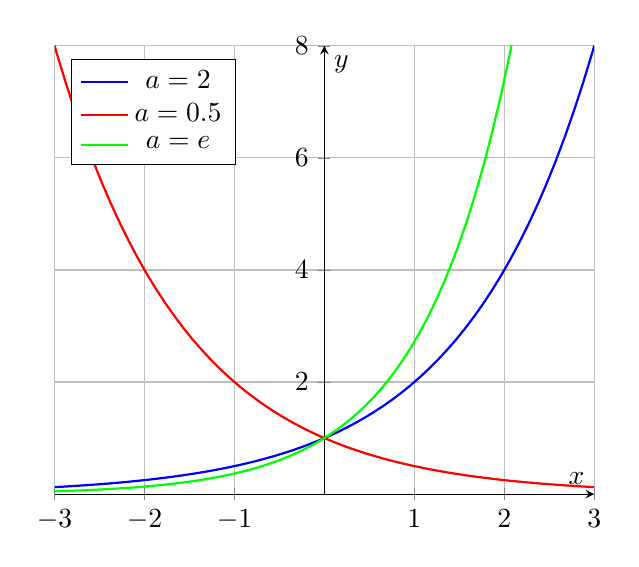
\begin{tikzpicture}
                \begin{axis}[
                    xmin=-3, xmax=3,
                    ymin=0, ymax=8,
                    axis lines=middle,
                    xlabel=$x$, ylabel=$y$,
                    grid=both,
                    samples=100,
                    legend pos=north west
                ]
                \addplot[blue, thick] {2^x};
                \addlegendentry{$a=2$};
                \addplot[red, thick] {(1/2)^x};
                \addlegendentry{$a=0.5$};
                \addplot[green, thick] {exp(x)};
                \addlegendentry{$a=e$};
                \end{axis}
            \end{tikzpicture}
        \end{column}
        \begin{column}{0.5\textwidth}
            \begin{itemize}
                \item 所有指数函数过点 \((0,1)\)
                \item \( a > 1 \) 时,函数图像向上增长
                \item \( 0 < a < 1 \) 时,函数图像向下趋近于 x 轴
                \item $x$ 轴是水平渐近线,也就是函数的值只能无限接近$0$.
                % \item 值域是$(0,+\infty)$
                % \item 定义域是$\mathbf{R}$,即 \( (-\infty, +\infty)\)
            \end{itemize}
        \end{column}
    \end{columns}
  \end{frame}
  
  
  \begin{frame}{定义域和值域}
    \begin{block}{定义域}
        指数函数 \( f(x) = a^x \) 的定义域是全体实数,即 \( (-\infty, +\infty) \)。
    \end{block}
    
    \begin{block}{值域}
        指数函数的值域是正实数集,即 \( (0, +\infty) \)。
    \end{block}
    
    \begin{center}
        \begin{tikzpicture}
            \draw[->] (-3,0) -- (3,0) node[right] {$x$};
            \draw[->] (0,-0.5) -- (0,3) node[above] {$y$};
            \draw[blue, thick, domain=-3:3] plot (\x, {exp(\x)/5});
            \draw[dashed] (-3,0) -- (3,0);
            % \node at (0,1.5) {值域:$(0,+\infty)$};
            % \node at (-2,0.2) {定义域:$(-\infty,+\infty)$};
        \end{tikzpicture}
    \end{center}
  \end{frame}
  
  
  \begin{frame}{单调性}
    \begin{columns}
        \begin{column}{0.5\textwidth}
            \textbf{当 \( a > 1 \) 时:}
            \begin{itemize}
                \item 函数严格递增
                % \item 导数 \( f'(x) = a^x \ln a > 0 \)
                \item 示例:\( f(x) = 2^x \)
            \end{itemize}
            
            \begin{tikzpicture}[scale=0.7]
                \begin{axis}[
                    xmin=-2, xmax=2,
                    ymin=0, ymax=4,
                    axis lines=middle,
                    samples=50,
                    xtick={-2,-1,0,1,2},
                    ytick={1,2,4}
                ]
                \addplot[blue, thick] {2^x};
                \draw[red, ->] (axis cs:0.5,1.5) -- (axis cs:1.5,3);
            \end{axis}
            \end{tikzpicture}
        \end{column}
        
        \begin{column}{0.5\textwidth}
            \textbf{当 \( 0 < a < 1 \) 时:}
            \begin{itemize}
                \item 函数严格递减
                % \item 导数 \( f'(x) = a^x \ln a < 0 \)
                \item 示例:\( f(x) = (0.5)^x \)
            \end{itemize}
            
            \begin{tikzpicture}[scale=0.7]
                \begin{axis}[
                    xmin=-2, xmax=2,
                    ymin=0, ymax=4,
                    axis lines=middle,
                    samples=50,
                    xtick={-2,-1,0,1,2},
                    ytick={1,2,4}
                ]
                \addplot[red, thick] {(0.5)^x};
                \draw[blue, ->] (axis cs:-1.5,3) -- (axis cs:-0.5,1.5);
            \end{axis}
            \end{tikzpicture}
        \end{column}
    \end{columns}
  \end{frame}
  
  
  
  
  \begin{frame}{总结}
    \begin{itemize}
        \item 指数函数 \( f(x) = a^x \) 的定义域为 \( (-\infty, +\infty) \),值域为 \( (0, +\infty) \)
        \item 单调性取决于底数 \( a \):\ \( a > 1 \) 时递增,\( 0 < a < 1 \) 时递减
        \item 所有指数函数过点 \((0,1)\)
  
    \end{itemize}
    
  \end{frame}
  
  
  \begin{frame}{题目1:指数运算化简}
    \begin{block}{题目}
        化简下列表达式:
        \begin{enumerate}
            \item $\frac{2^{3x} \cdot 4^x}{8^{x-1}}$
            \item $(3^{2x} \cdot 9^x)^{\frac{1}{2}}$
            \item $\frac{5^{x+1} - 5^x}{5^x}$
        \end{enumerate}
    \end{block}
    
    \begin{alertblock}{提示}
        利用指数运算法则:$a^m \cdot a^n = a^{m+n}$,$(a^m)^n = a^{mn}$,$\frac{a^m}{a^n} = a^{m-n}$
    \end{alertblock}
    \pause
      
      \begin{block}{答案}
          \begin{enumerate}
              \item $\frac{2^{3x} \cdot 4^x}{8^{x-1}} = \frac{2^{3x} \cdot (2^2)^x}{(2^3)^{x-1}} = \frac{2^{5x}}{2^{3x-3}} = 2^{2x+3}$
              \item $(3^{2x} \cdot 9^x)^{\frac{1}{2}} = (3^{4x})^{\frac{1}{2}} = 3^{2x} = 9^x$
              \item $\frac{5^{x+1} - 5^x}{5^x} = \frac{5^x(5-1)}{5^x} = 4$
          \end{enumerate}
      \end{block}
  \end{frame}
  
  
  
  \begin{frame}{题目2:指数方程求解}
    \begin{block}{题目}
        解下列方程:
        \begin{enumerate}
            \item $2^{x+1} = 32$
            \item $3^{2x} = 27^{x-1}$
            \item $4^{x} - 5 \cdot 2^{x} + 4 = 0$
        \end{enumerate}
    \end{block}
    
    \begin{alertblock}{提示}
        第3题可通过换元法转化为二次方程
    \end{alertblock}
    \pause
      
    \begin{block}{答案}
        \begin{enumerate}
            \item $2^{x+1} = 32 \Rightarrow 2^{x+1} = 2^5 \Rightarrow x = 4$
            \item $3^{2x} = 27^{x-1} \Rightarrow 3^{2x} = 3^{3x-3} \Rightarrow x = 3$
            \item 令 $t=2^x$,则 $t^2 - 5t + 4 = 0 \Rightarrow t=1$ 或 $t=4 \Rightarrow x=0$ 或 $x=2$
        \end{enumerate}
    \end{block}
  \end{frame}
  
  
  \begin{frame}{题目3:指数函数图像分析}
    \begin{block}{题目}
        已知指数函数 $f(x) = a^x$($a > 0$ 且 $a \neq 1$)的图像经过点 $(2, 9)$:
        \begin{enumerate}
            \item 求 $a$ 的值
            % \item 画出函数 $f(x)$ 的大致图像
            \item 指出函数的定义域、值域和单调性
            \item 比较 $f(0.5)$ 和 $f(1.5)$ 的大小
        \end{enumerate}
    \end{block}
    
    \pause
    
    \begin{block}{答案}
        \begin{enumerate}
            \item $a^2 = 9 \Rightarrow a = 3$
            % \item 图像:过点 $(0,1)$ 和 $(2,9)$,单调递增
            \item 定义域 $(-\infty,+\infty)$,值域 $(0,+\infty)$,在 $\mathbb{R}$ 上递增
            \item 根据单调性,故 $f(0.5) < f(1.5)$
        \end{enumerate}
    \end{block}
  \end{frame}
  
  
  
  
  \begin{frame}{题目4:指数函数定义域}
    \begin{block}{题目}
        求下列函数的定义域:
        \begin{enumerate}
            \item $f(x) = 2^{x^2 - 4}$
            \item $g(x) = \sqrt{1 - 3^x}$
            \item $h(x) = \frac{1}{4^x - 16}$
        \end{enumerate}
    \end{block}
    
    \begin{alertblock}{提示}
        考虑指数函数的底数限制以及分母不为零、偶次根号下非负等条件。
    \end{alertblock}
    
    \pause
    
    \begin{block}{答案}
        \begin{enumerate}
            \item 指数函数的指数部分为多项式,定义域为全体实数:$(-\infty, +\infty)$
            \item 根号内非负:$1 - 3^x \geq 0 \Rightarrow 3^x \leq 1 \Rightarrow x \leq 0$,故定义域为$(-\infty, 0]$
            \item 分母不为零:$4^x - 16 \neq 0 \Rightarrow 4^x \neq 16 \Rightarrow x \neq 2$,故定义域为$(-\infty, 2) \cup (2, +\infty)$
        \end{enumerate}
    \end{block}
  \end{frame}
  
  
  
  
  
  
  
  \begin{frame}{题目5:复合指数函数不等式}
    \begin{block}{题目}
        解不等式:
        \[
        2^{x^2 - 3x} > \left(\frac{1}{4}\right)^{x - 1}
        \]
    \end{block}
    
    \begin{alertblock}{提示}
        先统一底数,再利用指数函数单调性转化为代数不等式。
    \end{alertblock}
    
    \pause
    
    \begin{block}{答案}
        原不等式等价于:
        \[
        2^{x^2 - 3x} > 2^{-2(x - 1)} \implies x^2 - 3x > -2x + 2 \implies x^2 - x - 2 > 0
        \]
        解得:$x < -1$ 或 $x > 2$,即解集为 $(-\infty, -1) \cup (2, +\infty)$。
    \end{block}
  \end{frame}
  
  
  \begin{frame}{题目6:指数型函数的值域}
    \begin{block}{题目}
        求函数 $f(x) = 4^x + 2^{x+1} + 3$ 的值域。
    \end{block}
    
    \begin{alertblock}{提示}
        通过换元法转化为二次函数,注意新变量的取值范围。
    \end{alertblock}
    
    \pause
    
    \begin{block}{答案}
        令 $t = 2^x$,则 $t > 0$,函数化为:
        \[
        y = t^2 + 2t + 3 = (t + 1)^2 + 2
        \]
        当 $t > 0$ 时,$y$ 随 $t$ 增大而增大,故值域为 $(3, +\infty)$。
    \end{block}
  \end{frame}
  
  
  
  
  
  
  
  
  
  
  
  